\section{Question 1}
\subsection{Part a}
The development of perturbed EOMs around EPs can be found in many classical control text books, where each variable in the EOM is initially replaced by summation of two terms as follows and after the expansion, the nonlinear terms are eliminated while the steady state conditions are removed. In our case:
$$
x = x_e + \delta x, y = y_e + \delta y, z = \delta z
$$
Additionally, for simplicity we restrict our analysis in the xy plane where the primaries are located. The resulting perturbed EOM (about EPs) will be:
\begin{equation}
    \begin{cases}
        \delta \ddot{x} - 2\delta \dot{y} - \delta x &= -A\delta x+ B \delta y\\
        \delta \ddot{y} + 2\delta \dot{x} - \delta y & = C\delta x- D \delta y\\
    \end{cases}, \quad \text{where:} \begin{cases}
        A &= (1-\mu)\left(r_{1e}^{-3} - 3A_1\right)+ \mu\left(r_{2e}^{-3}-3A_2\right)\\
        B  &= 3(1-\mu)B_1 + 3\mu B_2\\
        C &= 3(1-\mu)B_1 + 3\mu B_2\\
        D &= (1-\mu)\left(r_{1e}^{-3} - 3C_1\right)+ \mu\left(r_{2e}^{-3}-3A_2\right)\\
    \end{cases}
\end{equation}
where:

\begin{align*}
    A_1 &= \dfrac{(x_e-\mu)^2}{r_{1e}^5}, \quad &A_2 &= \dfrac{(x_e-\mu+1)^2}{r_{2e}^5}\\
    B_1 &= \dfrac{(x_e-\mu)y_e}{r_{1e}^5}, \quad &B_2 &= \dfrac{(x_e-\mu+1)y_e^2}{r_{2e}^5}\\
    C_1 &= \dfrac{y_e^2}{r_{1e}^5}, \quad &C_2 &= \dfrac{y_e^2}{r_{2e}^5}\\
\end{align*}
As expressed above, the constants A, B, C and D can be determined (based on the EPs coordinates) and the three body system under consideration.

In the canonical system, the L4 coordinates are given below. Putting this information in the perturbed EOMs yields:
\begin{equation}
    L4 = \begin{cases}
        x_e = \mu - 0.5\\
        y_e = \dfrac{\sqrt{3}}{2}
    \end{cases}, \quad \begin{cases}
        r_{1e} = 1\\
        r_{2e} = 1
    \end{cases}
\end{equation}
\begin{equation}
    \begin{cases}
        \delta \ddot{x} - 2\delta \dot{y} - \dfrac{3}{4}\delta x - \dfrac{3\sqrt{3}}{4} \left(\mu-\dfrac{1}{2}\right)\delta y = 0\\
        \delta \ddot{y} + 2\delta \dot{x} - \dfrac{3\sqrt{3}}{2}\left(\mu-\dfrac{1}{2}\right)\delta x - \dfrac{9}{4}\delta y = 0\\
    \end{cases}
\end{equation}
where:
\begin{equation}
    R_1\delta \ddot{r} + R_2\delta \dot{r} + R_3\delta r = 0
\end{equation}
where:
\begin{equation}
    R_1 = \begin{bmatrix}
        1 & 0\\
        0 & 1 \end{bmatrix}, \quad R_2 = \begin{bmatrix}
        0 & -2\\
        2 & 0 \end{bmatrix}, \quad R_3 = \begin{bmatrix}
        -\dfrac{3}{4} & -\dfrac{3\sqrt{3}}{2}\left(\mu-\dfrac{1}{2}\right)\\
        -\dfrac{3\sqrt{3}}{2}\left(\mu-\dfrac{1}{2}\right) & -\dfrac{9}{4} \end{bmatrix}
\end{equation}

One can assume an exponential solution to determine the system characteristic equation, out of which the eigenvalues can be determined for stability analysis. So let $\delta r =  ae^{\lambda t}$ where a
is a constant matrix. Substituting this solution in the perturbed EOMs for L4, will give:
\begin{equation}
    \begin{vmatrix}
        \lambda^2 - \dfrac{3}{4} & 2\lambda - \dfrac{3\sqrt{3}}{2}\left(\mu-\dfrac{1}{2}\right)\\
        2\lambda - \dfrac{3\sqrt{3}}{2}\left(\mu-\dfrac{1}{2}\right) & \lambda^2 - \dfrac{9}{4}
    \end{vmatrix}a = 0
\end{equation}
The expression is an eigenvalue or eigenvector problem.
After simplifying, the determinant of the above equation one would get:
\begin{equation}
    \lambda^4 + \lambda^2 - \dfrac{27}{4}\mu(\mu-1) = 0\xrightarrow{\text{solving for} \lambda^2}\lambda^2 = \dfrac{-1\pm\sqrt{1+27\mu(\mu-1)}}{2}, \quad 0 \leq \mu \leq 1
\end{equation}
Neutral stability requires all $\lambda$'s to be imaginary, as it is not possible to obtain four roots with negative real parts for L4. Then for stability it must be:
\begin{equation}
    \mu < \mu_1 = 0.03852, \quad \mu > \mu_2 = 0.96148
\end{equation}
In jupter system, $\mu = 0.00095$ which is less than $\mu_1$ and therefore L4 is stable in this system.
\subsection{Part b}
In this section used Code from github and source code is is Code/Q1 directory. Here is the jaccobi constant plot for the Sun jupter system.
\begin{figure}[H]
    \centering
    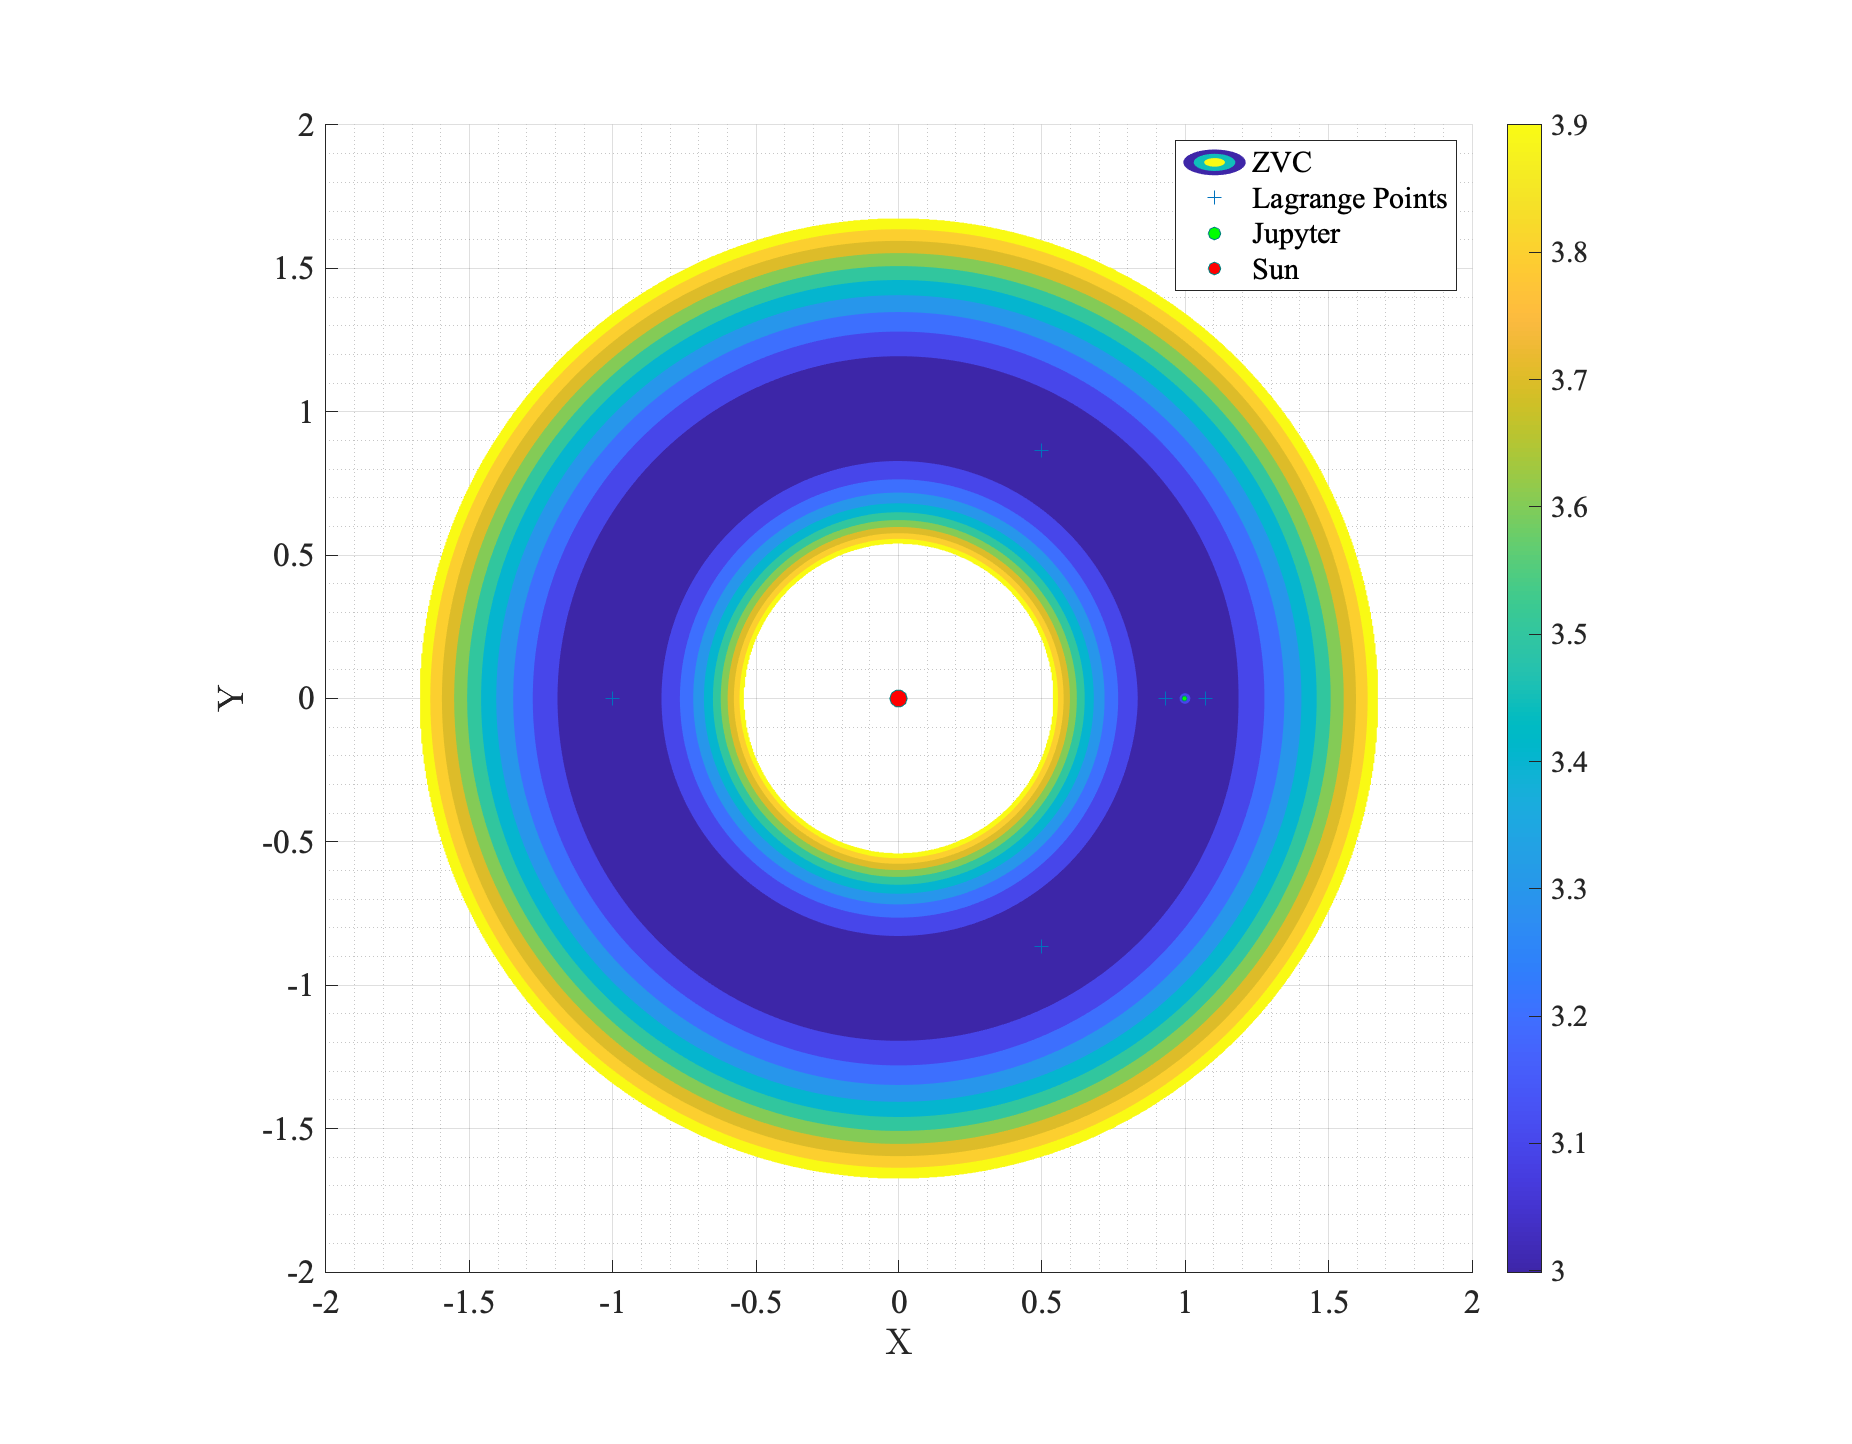
\includegraphics[width=\textwidth]{../Figure/Q1/jaccobi_1}
    \caption{Jaccobi constant plot for the Sun jupter system with fiiled countour for lagrange points}
    \label{fig:my_label}
\end{figure}

\begin{figure}[H]
    \centering
    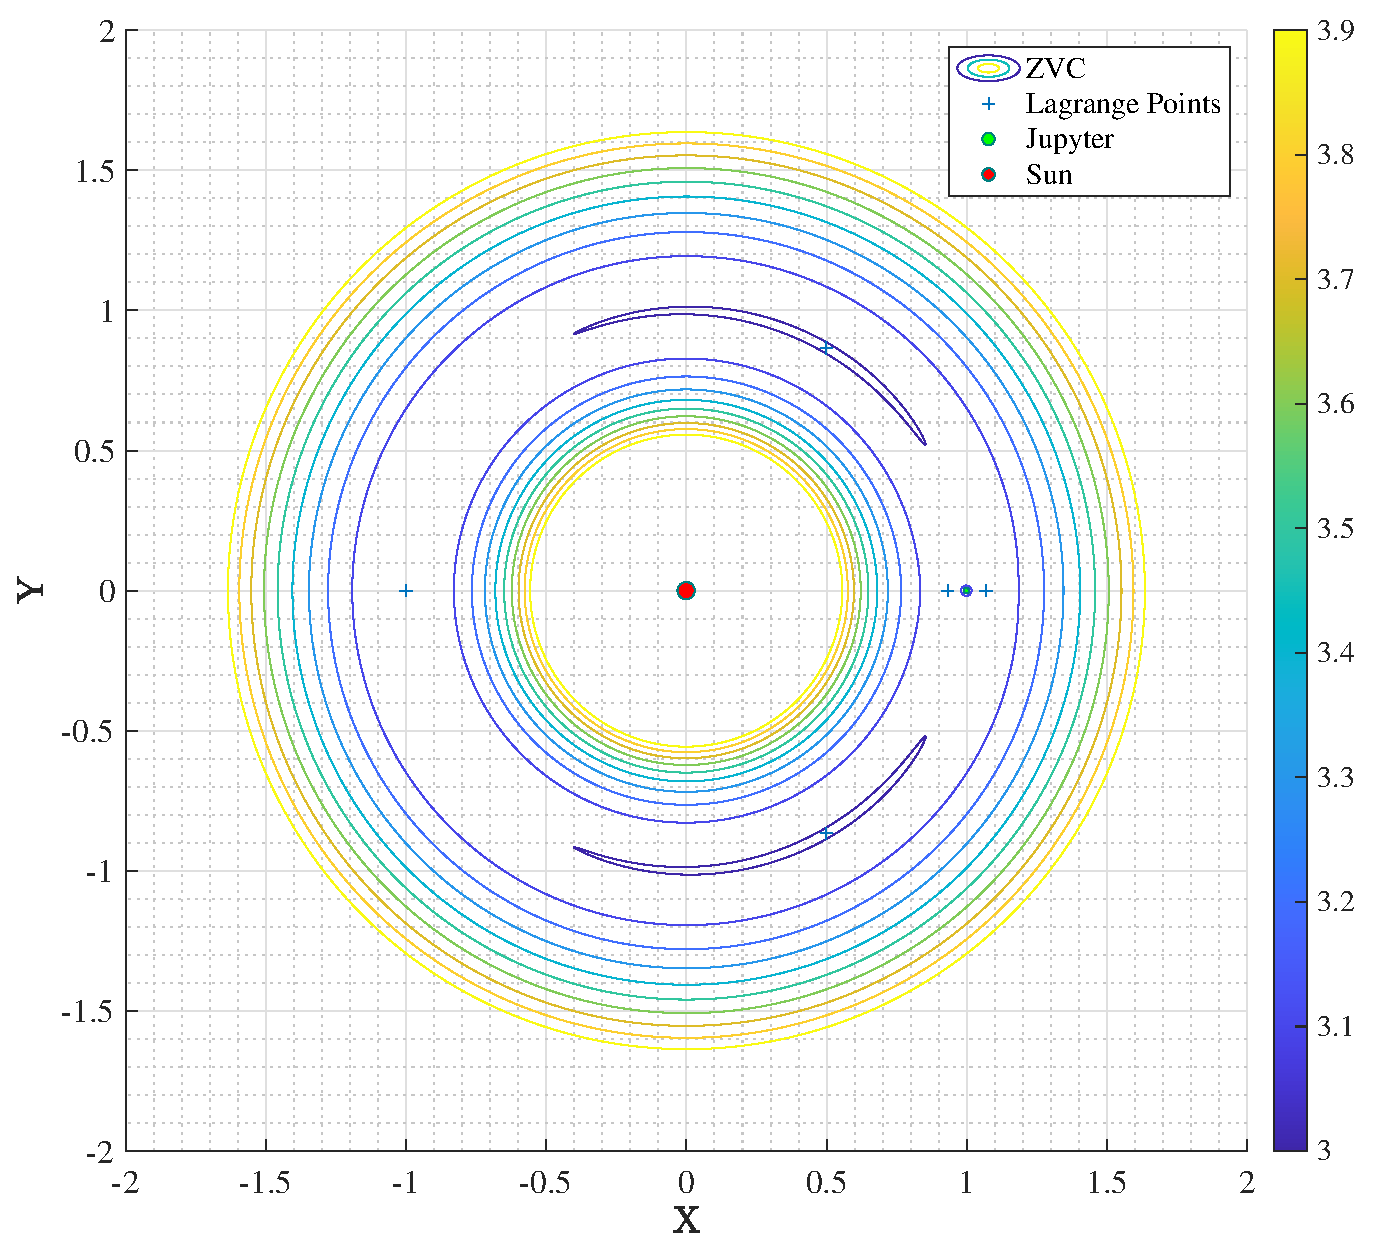
\includegraphics[width=\textwidth]{../Figure/Q1/jaccobi_2}
    \caption{Jaccobi constant plot for the Sun jupter system countour for lagrange points}
\end{figure}
